\documentclass[conference]{IEEEtran}
\IEEEoverridecommandlockouts
% The preceding line is only needed to identify funding in the first footnote. If that is unneeded, please comment it out.
\usepackage{cite}
\usepackage{amsmath,amssymb,amsfonts}
\usepackage{graphicx}
\usepackage{textcomp}
\usepackage{xcolor}

% folder gambar
\graphicspath{{./figures/}}


\def\BibTeX{{\rm B\kern-.05em{\sc i\kern-.025em b}\kern-.08em
    T\kern-.1667em\lower.7ex\hbox{E}\kern-.125emX}}

\begin{document}

\title{Vehicle Tracking and Theft Detection System}

\author{
\IEEEauthorblockN{Puji Valen Crisgar\textsuperscript{1}, Patrick Ryan Wijaya\textsuperscript{2}, Marcell D. F. Pakpahan\textsuperscript{3},\\ Eniman Yunus Syamsuddin\textsuperscript{4}, Muhammad Ogin Hasanuddin\textsuperscript{5}}
\IEEEauthorblockA{\textit{School of Electrical Engineering and Informatics} \\
\textit{Institut Teknologi Bandung}\\
Bandung, Indonesia \\
Email: \{\textsuperscript{1}13217013, \textsuperscript{2}13217027, \textsuperscript{3}13217082\}@std.stei.itb.ac.id, \textsuperscript{4}eniman@stei.itb.ac.id, \textsuperscript{5}moginh@itb.ac.id}
}



\maketitle

\begin{abstract}
The proposed Vehicle Tracking System is designed upon the ESP32 architecture to locate the coordinates of the vehicle, alongside being able to detect an unwanted movement of the vehicle, and vehicle engine turning on unexpectedly, indicating an act of theft. Data and telemetry are transmitted through the Internet via mobile network, while location detection relies on a GPS module with an external Antenna. Data is Transmitted via MQTT Protocol through Google Cloud IoT Core, where it will be delivered to Firestore Database available from Google Firebase. The data can be monitored by the owner of the vehicle via a Progressive Web App-based User Interface, also built upon Firebase, which will be able to control the modes of the device, display the real-time location of the vehicle via Google Maps, a collection of historical data of the vehicle’s movement, and alert the user via notification when theft action is detected.
\end{abstract}

\begin{IEEEkeywords}
GPRS, GSM, IoT, ESP32, Firebase, PWA
\end{IEEEkeywords}

\section{Introduction}
Internet-of-Things (IoT) has allowed humans to create solutions to problems which were not available. The ability for devices to connect and "talk" to 
each other and share information has allowed new levels of interconnectivity between all of us. IoT devices themselves have come a long way in terms of the development and accessibility, with new devices with different features becoming available for the general public to access and experiment with. 
One of the key uses of IoT is to design a vehicle tracking system to solve the issue of not knowing where the location of someone's vehicle is,
and detecting a possible act of theft to the vehicle. 

The main technology used in this system to detect the location of the vehicle is GPS. GPS, also known as Global Positioning System, is a system built upon satellites 
to pinpoint the location of an object with a GPS receiver in the form of Longitude and Latitude. These data can be collected via a device that is planted in the vehicle, 
which hosts a GPS receiver and used accordingly to give the user information regarding the location of the device. Representation of the data can be formulated to an interactive
visual interface instead of numerical longitude and latitude values through available interactive mapping resources such as Google Maps and OpenStreetMap. Transmission of data from 
the device can use different technologies, such as mobile telecommunications interface (GPRS, 3G, LTE), LoRa, NB-IoT. However, 
with mobile telecommunications network offering the biggest coverage of area, especially in the country of Indonesia, and factoring in costs of production of the proposed device, 
GPRS mobile telecommunications network is used in this project to send data from the device to the user's end.

The ability to detect the location of the vehicle will also be paired with the ability of the device to detect a possible theft attempt. Detection is done through scanning for unwanted engine starts, and through 
detection of the change of the vehicle's location past a certain distance threshold. To avoid minimizing false positive results, the user will have to set the device to a certain configuration, therefore scanning 
and detection of those parameters will only be done when the device is set to this very configuration. Control of the device will be done via a web application, where do the user will
be able to view the location of the device from an Interactive Map platform and follow real time updated gathered from the device. All of the infrastructure needed to execute end-to-end functions (from device to user) 
will use Google Cloud features, which include Google Firebase, IoT Core, Cloud Functions and Google Maps API, which is chosen to enable seamless integration and eliminate possible compatibility issues.

\section{Related Works}
Due to high demand of such systems, there has been several previous attempts to design a vehicle Tracking system, all has involved the use of GPS, with GPS receivers being the component to use and integrate in the device. 
One previous attempt involved the system sending location data 
in the form of Short Message Service (SMS) to alert the user regarding real time location of the vehicle, as well as detection of theft. Detection of theft is done through an RFID sensor to detect an event of engine 
turning on. Data is then presented via Google Maps link that will redirect the user to an external Google Maps application to view the location. Control such as commands to the device are done manually through the SMS 
via specific text-based commands \cite{iotmounika}.
Another attempt in designing a vehicle tracking system involves the design of Java-based system to allow users to interact and retrieve positional data from the device, while still using SMS-based messages to control the 
configuration of the device in the event of a position information request. Location data is sent via TCP socket through GPRS network to be stored in a database \cite{6132526}. 
Another system was designed to be accessed with a mobile-based application running specifically on iOS hardware, where the location data is displayed via Google Maps, but without any capabilities to detect any attempt of theft, and is used 
solely for vehicle location tracking. The referenced system uses GPRS as a method of communication while GPS is used for location detection \cite{6803187}.
Lastly, a system was designed using the basic architecture of a GPS receiver while integrating the use of a cut-off switch to be able to turn off
the vehicle's power once it has detected an act of theft. The detection of the act of theft still needs confirmation from the user on whether it is a true-positive / false-positive detection, every time the 
vehicle engine turns on. Once the user has confirmed this act of theft, the cut-off switch will then turn the car off and the system will be able to deliver the location of said vehicle \cite{article1}. 

\section{Proposed System}
The paper presents a system which is designed to locate the vehicle location using GPS and GPRS technology via hardware planted on the user's vehicle. The system will be based on Espressif ESP32 Controller to handle the operations of the devices, 
with integrated SIMCOM SIM800L GSM/GPRS Module to be able to communicate with the network to transmit information to the user. GPS capabilities will be handled by a separate GPS receiver to acquire latitude and 
longitude values. In order for the system to be able to power itself, while also detecting an act of car theft, the device will interface with the On-board diagnostics (OBD) port of the vehicle, where it will 
receive constant voltage to power the device, while also receiving data in the form of impulses which will be detected by the device to determine an engine start event. Besides that, the device will be able to detect if it is unplugged from the 
OBD Port, where an emergency power source in the form of rechargeable Lithium-Ion Batteries will be used to power the device for a certain period of time. 

All the information gathered from this device will then be transmitted via Internet through GPRS network provided by support network providers. For data to be received to the end user, it will have to travel to different stages. The first 
part of the transmission involves the data being sent to Google Pub/Sub Client, which is a part of Google IoT Core services. The device will communicate with Pub/Sub Client via MQTT, a lightweight communications protocol to enable low power data communications 
to minimize power consumption, especially in the situation where emergency power is used. 

On the other side, the user will interact with a web application design as a Progressive Web App (PWA), able to be accessed in different devices with access to a web browser. 
The decision to create a user interface based on PWA is that it enables implementation of features such as push notifications and native user experience for iOS and Android systems running on smartphones, 
while being more lightweight in terms of file size and processing power usage compared to traditional apps \cite{8456349}. Lastly, PWA allows the app to be compatible with a wider range of devices with minimal changes needed to 
each platform, thus minimizing development time of the user interface. This web-based application will then be hosted with Firebase, where it will use Firebase features such as Firebase Authentication for user account management needs, 
Firebase Cloud Messaging for enabling push notifications, and Firebase Firestore as the main database backing up the web app. The PWA will allow the user to do multiple things, which include: create/sign in to their account, pair/link the devices to the respective accounts, view the current location of the device via Google Maps API, enable/disable Realtime Tracking Mode, enable/disable Theft Monitoring Mode and view recorded historical data of the device. 

To integrate the communication of both the device and the user, Google Cloud Functions will be used to create functions that will run whenever a certain event has occurred. These functions will be explained further in the coming segments, but will include, but not limited to : 
save incoming data from device to Firebase Firestore, pass through commands to enable and disable both Realtime Tracking Mode and Theft Monitoring Mode to the device and pairing said device to a specific user account. Thus, it can be inferred that Cloud Functions will be the 
backbone of the system in order for both the device and user to communicate and exchange data with each other. To better visualize the system, the system can be presented into a system diagram as shown below. 

\begin{figure}[htbp]
    \centering
    \includegraphics[width=0.45\textwidth]{skematikdiagram1}
    \caption{Overview of The System}
    \label{fig1}
\end{figure}

\section{Tracker Subsystem}
Tracker Subsystem is the subsystem that will do data acquisition on location, theft detection and other data such as network status and GPS signal availability. 
The process of development for this subsystem is done using Mongoose OS platform. Mongoose OS is development framework focused on IoT aspect and allows for seamless and easier 
integration to cloud infrastructure such as Google Cloud, Amazon AWS and Azure IoT. It supports multiple devices such as ESP32 and ESP8266, where ESP32 will be used in this system.
\begin{figure}[htbp]
    \centering
    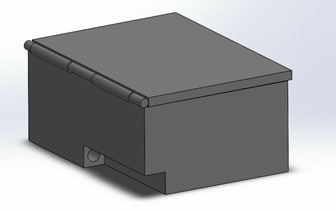
\includegraphics[width=0.45\textwidth]{casing1}
    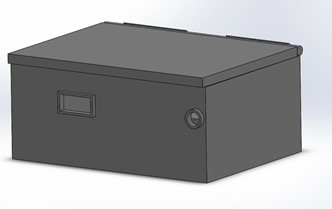
\includegraphics[width=0.45\textwidth]{casing2}
    \caption{Physical Features of Tracker Device}
    \label{fig1}
\end{figure}
\begin{figure}[htbp]
    \centering
    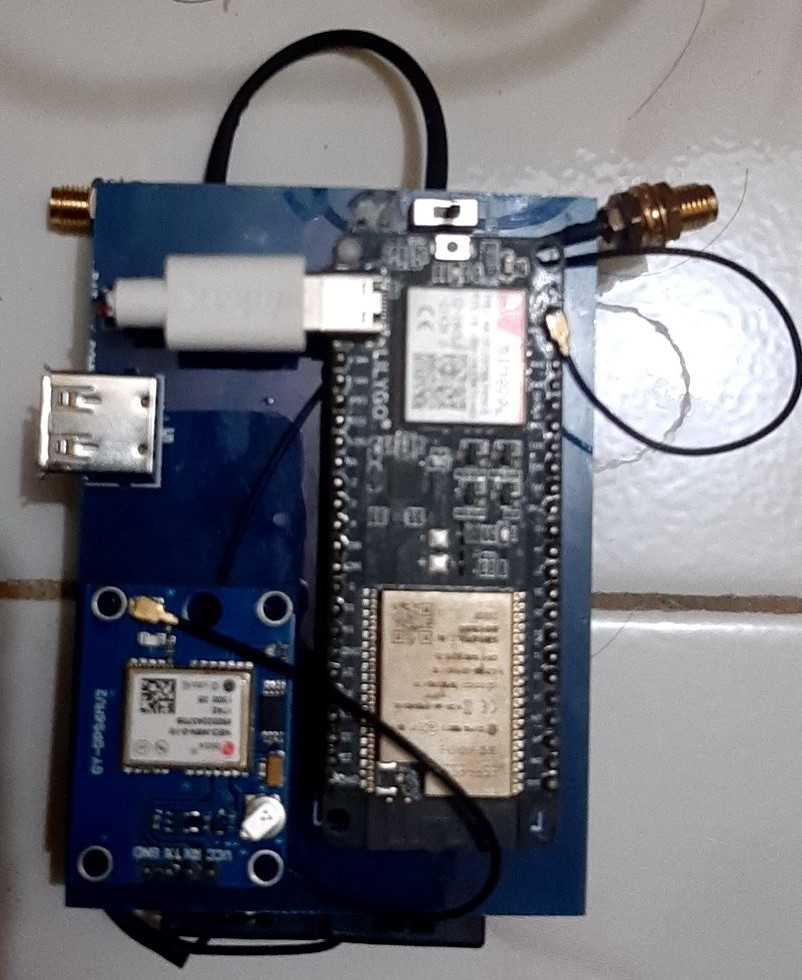
\includegraphics[width=0.3\textwidth]{fotoalat}
    \caption{Internal View of Tracker Device}
    \label{fig1}
\end{figure}
\subsection{Data Processing and Communications Module}
Data Processing Module consists of TTGO-TCall ESP32 Module. This Module has integrated SIM800L module that will act as mobile modem to connect to telecommunications 
mobile network. It also includes IP5306 System-on-Chip (SoC) to power up the board using battery, and controls battery charging process. This board allows for 
conventional communication between module via GPIO pins that are available, and providing power pins to modules such as GPS Module.

The included SIM800L module has capabilities of connecting to 2nd generation or GPRS mobile network. 3G and 4G-based modules are considered when designing the system. However, 
the cost associated with these modules and the availability in acquiring them in Indonesia, has made it impossible to design the system using said modules in the given timeframe. 
Besides that, SIM800L has had a wide range of support with the IoT community and therefore eases the development process with multiple sources of help available online.

\begin{figure}[htbp]
    \centering
    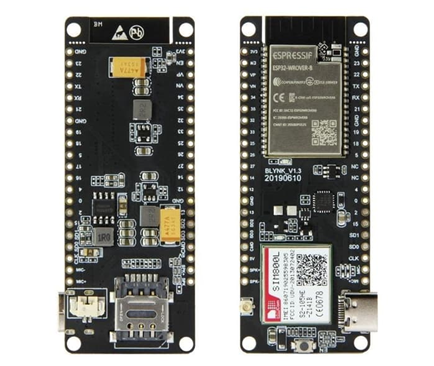
\includegraphics[width=0.45\textwidth]{gambaresp32}
    \caption{TTGO T-Call ESP32 Board with integrated SIM800L Communications Module}
    \label{fig1}
\end{figure}

\subsection{Location Sensing Module}
The functionalities of coordinate data acquisition for real time tracking and historical data collection is fulfilled by u-Blox NEO-6M Module. NEO6M module is a GNSS receiver with capabilities of receiving 
from US GPS satellite network. Compared to newer variants from u-Blox, notably the M8 Series receivers, the NEO-6M lacks the ability to receive data from Galileo and GLONASS satellite networks. However, as with 
the choice of SIM800L module for communication, the availability and price of the module are the key reasons on why NEO-6M is used.

NEO-6M Module is powered by an on-board 3.3V power source from the ESP32 module. Communication between NEO-6M Module and ESP32 module are as follows:
\begin{itemize}
\item 'Tx' Pin on NEO-6M connects to pin 'GPIO14' of ESP32module.
\item 'Rx' Pin on NEO-6M connects to pin 'GPIO12' of ESP32module.
\end{itemize}
The original Rx and Tx pins available at ESP32 Module cannot be used and therefore arbitrary GPIO pins must be used. The reason of this will be explained later during software development explanation.

\begin{figure}[htbp]
    \centering
    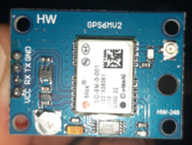
\includegraphics[width=0.2\textwidth]{neo6m}
    \caption{u-blox NEO-6M Module}
    \label{fig1}
\end{figure}

\subsection{Theft Detection Data Acquisition Module}
Theft detection is possible when the user selects a mode/configuration that will monitor the following 2 scenarios: 
\begin{itemize}
\item When the vehicle is detected as moving from its original position where the user initially turns on the configuration.
\item When the vehicle engine turns on.
\end{itemize}
The first scenario can be fulfilled from comparing location data that has been acquired. The second scenario, however, will need 
additional interfacing modules to gather more information. This information is the information of the car being on or off. To get this data, 
the device will interface with the vehicle with On Board Diagnostics (OBDII) Port. OBDII Port are mandatory features that can be found in cars. 
While different cars have different standards for their OBDII ports, where each port can send different types of data, it is crucial for this 
system to be used in types of cars. Therefore, detection of engine turning on is done by monitoring for impulses in the data lines of the individual pins, 
where the data pins will be active only once the engine of the car is turned on. From this detection, the current from the data line being active will be converted 
have its voltage dropped to around 3.3V using a DC-DC Converter and connected to a GPIO pin, and thus detect 
if engine is running during this monitoring configuration. Aside from this functionality, OBDII port will supply power to the device, where the 12 V supply available from the port
will be converted using a DC-DC Converter to 5V which will then be used by the device to power itself, and charge the on-board backup battery. 
\begin{figure}[htbp]
    \centering
    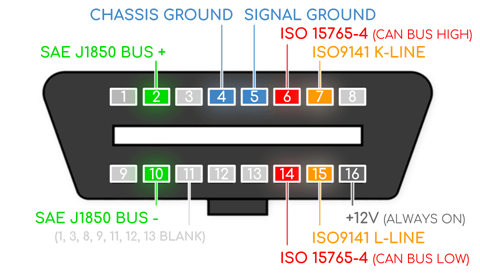
\includegraphics[width=0.45\textwidth]{obddiagram}
    \caption{Pinout Diagram of an OBDII Port}
    \label{fig1}
\end{figure}
Another feature that will be available is the ability to detect if the device is plugged into the OBDII port or not. This can be achieved by detecting the sudden missing availability of 
power supply from OBDII Port when the device is plugged off. This will then be notified to the user. The user will then be able to use this information depending on the situation, especially if 
the vehicle has been left to park and the message appears, providing one more layer of security in case the theft detection triggers fail.


\subsection{Backup Power Module}
The system designed will have a backup power module in the form of rechargeable Lithium-Ion Batteries. These batteries need to be able to last a certain period of heavy usage in the case of the device being unplugged from the OBDII port. 
The system uses 2 3400 mAh Panasonic NCR18650B batteries, totaling the capacity to 6800 mAh. This will be connected via a proprietary connector available in the ESP32 module, and charging will be managed by IP5306 SoC module as mentioned 
previously. 
\begin{figure}[htbp]
    \centering
    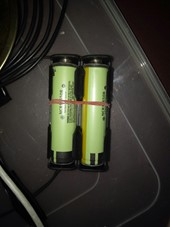
\includegraphics[width=0.25\textwidth]{bateri}
    \caption{Panasonic NCR18650B}
    \label{fig1}
\end{figure}

\section{Cloud Subsystem}
Google Cloud will be the provider of the Cloud infrastructure, where multiple solutions offered by Google Cloud will work together to perform the function of transporting data from Tracker to User Interface, and vice versa. 
Google Cloud solutions that will be used are as follows:

\subsection{Google Cloud IoT Core}\label{AA}
Cloud IoT Core allows for securely connecting and managing IoT devices to the Google Cloud Infrastructure, and acts as the connecting bridge of these devices to other Google Cloud Solutions \cite{iotcorewebsite}. Devices connect to IoT Core via registry that 
is created from Google Cloud Console. This registry, when devices are connected, will be able to show a full log of input and output of the device, or the CONFIG and STATE of the device in relation to the display of the device in the log. 
\begin{figure}[htbp]
    \centering
    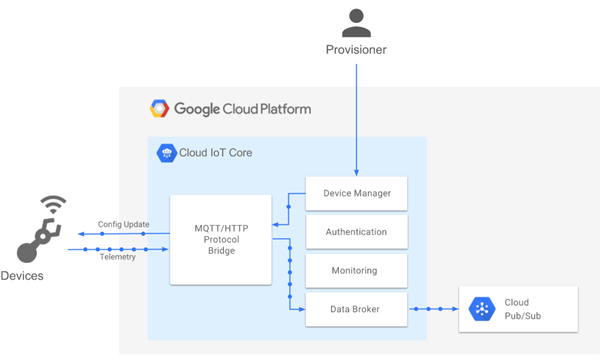
\includegraphics[width=0.45\textwidth]{iotcorediagram}
    \caption{Google IoT Core Data Movement}
    \label{fig1}
\end{figure}
As seen from the figure above, the device communicates via MQTT Secure Protocol via a Protocol Bridge, where this protocol will also allow communication between the server side in terms of changing configuration on deliver this to the device. 
Data from device is then sent to a Pub/Sub bucket specifically made for the created registry and this data can be accessed and used by other Google Solutions such as Cloud Functions.

\subsection{Cloud Functions}
Cloud Functions allows triggering of certain methods and functions via different solutions that are available at Google Cloud, where data from a solution can be used by another solution. One example of this is triggering a function from a change in Firestore 
Database, or triggering a change in Pub/Sub Bucket to activate certain functions \cite{cloudfunctionwebsite}. In this case. Cloud function will be used for the following:
\begin{itemize}
\item Store telemetry sent from Tracker to Firestore Database, triggered by a new publish of Data from Pub/Sub Client of the Created IoT Core Registry
\item Send configuration updates from User Interface to change the modes of the Tracker, triggered by an HTTPS request from the front end (i.e. press of a button available in the user interface)
\item Pair a device with a user account in order for it to be accessed by said account, triggered by an HTTPS request from the front end
\item Send push notifications based on change in Firestore document data, triggered by a change of data in the field of a Device Document in Firebase Firestore
\end{itemize}
Cloud functions thus allows the developer to build serverless backends as the process of creating a single Cloud Function involves defining the function itself in the form of an index JavaScript file. Deploying these functions would just require a single command 
and once these functions are deployed, that can be used instantly. This greatly reduces the development time of the project, while still allowing the system to perform the desired capabilities and behaviors.  
\begin{figure}[htbp]
    \centering
    \includegraphics[width=0.45\textwidth]{skematikdiagram2}
    \caption{Cloud Functions in Relation to Other Subsystems}
    \label{fig1}
\end{figure}

\subsection{Firebase Firestore}
Firebase Firestore is a NoSQL-based database offered by Google Firebase that can be accessed by Firebase applications as well as other Google Solutions such as Cloud Functions, and enables Firebase applications to access real time data, and allows updates of real time data 
to be served to the user from different platforms. Firebase Firestore stores data in the form of collection and documents. A collection may contain several documents, and a document can be linked to a number of collections as well. A document can store different types of data 
distinguished by fields that can be set by the developer. The structure of the database used in this project can be shown below: 

\begin{figure}[htbp]
    \centering
    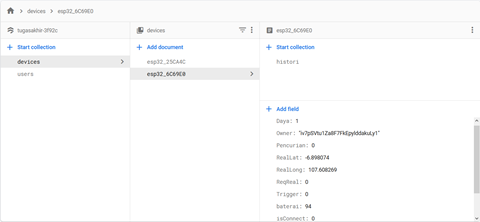
\includegraphics[width=0.45\textwidth]{strukturdatabase1}
    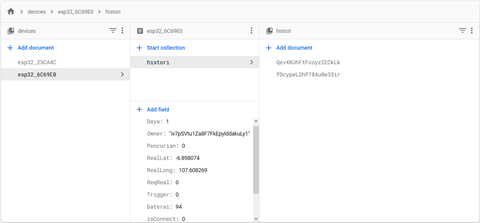
\includegraphics[width=0.45\textwidth]{strukturdatabase2}
    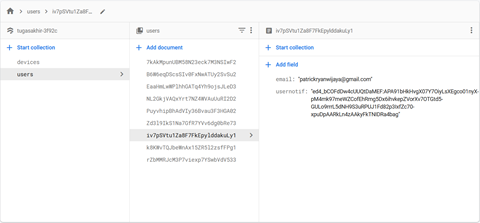
\includegraphics[width=0.45\textwidth]{databaseuser}
    \caption{Structure of Firestore Database for the System}
    \label{fig1}
\end{figure}

The figure above shows that the database can be divided in two main collections: 'devices' and 'users'. the collection 'users' contain documents of all the registered users, containing email data and notification tokens to be used for receiving notifications. The name of the document uses 
the randomly generated user ID from Firebase Authentication. the collection 'devices' contain documents of all the registered and activated tracker devices, where the name of each document correspond to the name of tracker that is created when device is connected to Google IoT Core. This is to 
make sure that the data sent from a specific device will arrive to the correct document with the same name. The document itself contains several fields, consisting of: real time longitude and latitude; owner of the tracker, which corresponds to the user ID that is generated and used by Firebase 
Authentication to identify a user; the fields 'Trigger' and 'ReqReal' containing values of either '0' or '1', which will be identified by the Tracker to be used to change the configuration of the device; the fields 'isConnect', 'isGPS' and 'baterai' corresponding to mobile data connection status, GPS data 
availability and battery level respectively; the fields 'Daya' and 'Pencurian' to identify whether the device has been plugged off from the OBDII port and to identify if the vehicle has been stolen, respectively. These data will be used from each side of the system (Tracker side and User Interface Side) by 
Cloud Functions and create a communication system between these two ends. Linked to the Tracker Document is a collection of historical data that will contain historical data documents. These historical data documents consist of latitude, longitude and timestamp data to differentiate themselves from each other. The 
user will be able to access this information in the user interface.

\section{User Interface Subsystem}
This subsystem will be responsible for the user’s interaction, which includes account management functionalities such as creating and accessing accounts, receiving push notifications in regard to events such as theft detection and the unplugging of OBDII port, pairing trackers with an account, as well as a method in which to access data received from device to a presentable visual form. 
This subsystem will also allow the user to control different configurations of the device, in order to change the behavior of the device. The user interface is built as a Progressive Web App, essentially a website with a service worker to implement functions such as offline caching and notification event listening. Progressive Web Apps also allow the user to install the application as if the program 
is a native application for each respective device, currently supported in Windows 10, iOS and Android devices. 

This subsystem consists of multiple pages, each performing a different task. Login page will be used for both creating a new account and login to an existing account. Dashboard page will be the main page to access telemetry Data such as real time location, availability of mobile network and GPS data, and backup power reserve percentage. Dashboard also allows initial pairing of device to the account.
History page will be used to access historical data of each paired device. All of the location data will be displayed via Google Maps and shown in relation with the current location of the user via their geolocation data. 

\subsection{Firebase Authentication}\label{AA}
Firebase Authentication will be used to handle account management request, such as creating an account, verifying an account and accessing an already created account. Firebase Authentication allows a simple implementation of authentication as it is in the form of a ready-to-use function that can be called from the Firebase Authentication SDK. Firebase Authentication allows multiple methods of 
account creation, such as Google Account Login or Facebook Account Login.
In this system, the user can create an account with an email, then set a password and lastly will be able to verify their account via email verification. Users who are able to verify their accounts 
can log in and access the Dashboard page where the user will be able to add/pair activated trackers. The figure below the design of the User Interface for register and login processes.
\begin{figure}[htbp]
    \centering
    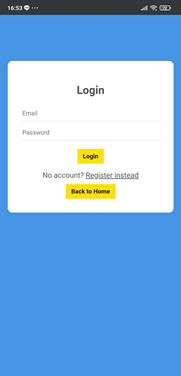
\includegraphics[width=0.2\textwidth]{tampilanlogin}
    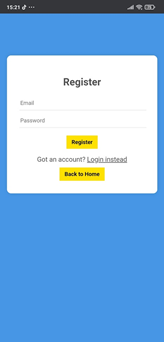
\includegraphics[width=0.2\textwidth]{tampilanregister}
    \caption{Login and Register User Interface}
    \label{fig1}
\end{figure}

\subsection{Firebase Cloud Messaging}
Firebase Cloud Messaging allows the function of implementing push notifications to users, by working together with Service Worker of the Progressive Web App application, and Cloud Functions to send notifications such as a warning that the vehicle has been stolen, and a message regarding disconnect of device from OBDII port. 
Firebase Cloud Messaging uses tokens to trigger notifications, where the tokens will be given to a user when accessing the Dashboard page. This token will be saved in Database in the user's document section of the database. Notification will be triggered once an event happened, in this case a change on the fields of the Tracker document as mentioned previously. 

\subsection{Firebase Hosting}
Firebase Hosting will be used to serve all the resources of the application, and thus accessible via domain. One of the key advantages of using Firebase Hosting is the ability to serve securely via HTTPS and therefore communication between the user and the server is encrypted. 
Firebase hosting also allows deployment of different versions of the application, which is useful in a situation where a new deployment can cause problems, and a quick 'undo' action is necessary to make sure the user's experience will not be interrupted by the problematic deployment.

\subsection{Google Maps API}
Google Maps API will be used to visually display the coordinate data received from the Tracker Device. Google Maps is implemented using Maps JavaScript API that is available to be used using an API key generated on Google Cloud Console. Alongside the location data of tracker will also be the location 
of the user, who will use the geolocation data of the device used to access the user interface (i.e. mobile phone or desktop device). Maps API will be used to display both real time location and historical location.

\section{Results}
Results will be broken down to 5 main segments: the accuracy of tracker; creating and accessing an account; pairing the device to an account; doing real time tracking and historical location data collection; theft detection simulation. 

\subsection{Creating and Accessing an Account}
The user can create an account using a valid email address and password. Valid email address refers to it being a genuine contactable email address and has not been used to create an account. The user will then be able 
to receive an email containing a link to verify their account. The process can be viewed in the figures. 
\begin{figure}[htbp]
    \centering
    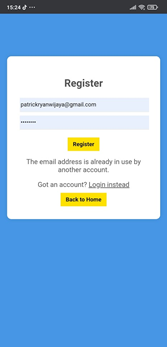
\includegraphics[width=0.2\textwidth]{registerfail1}
    \caption{Data Validation During Registration Process}
    \label{fig1}
\end{figure}
\begin{figure}[htbp]
    \centering
    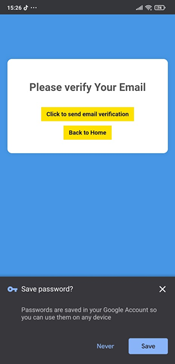
\includegraphics[width=0.2\textwidth]{emailver1}
    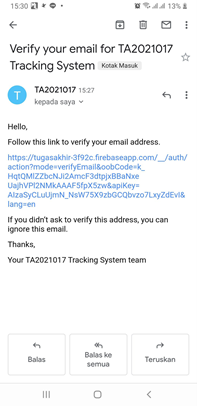
\includegraphics[width=0.2\textwidth]{emailver2}
    \caption{Account Verification Process}
    \label{fig1}
\end{figure}
Once the user is able to verify their account, they will be able to log in with the log in form available in the user interface. The user will be asked to enter a valid email address and password. Valid email address in this case refers to 
an email address that has previously been used to register to the system. Besides that, the system will check for the password to make sure that the password for the account is correct. Once the user 
is able to log in, they will be redirected to the Dashboard. 
\begin{figure}[htbp]
    \centering
    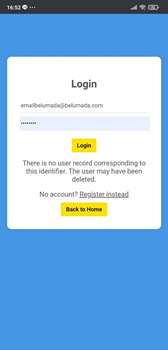
\includegraphics[width=0.2\textwidth]{loginfail1}
    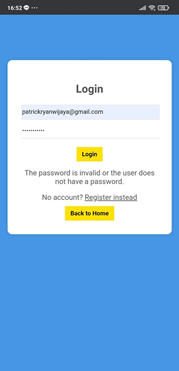
\includegraphics[width=0.2\textwidth]{loginfail2}
    \caption{Data Validation During Login Process}
    \label{fig1}
\end{figure}
\begin{figure}[htbp]
    \centering
    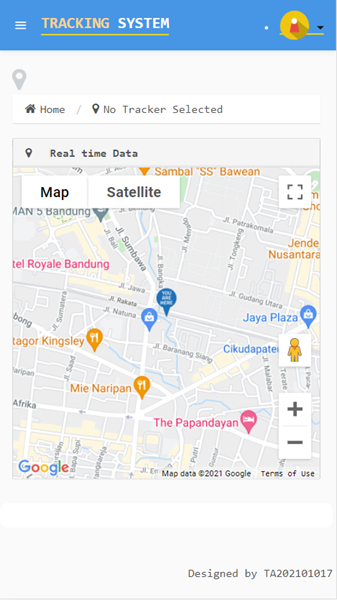
\includegraphics[width=0.2\textwidth]{tampilandashboard}
    \caption{User will be directed to Dashboard Page after Successful Login Attempt}
    \label{fig1}
\end{figure}

\subsection{Pairing an Account with Tracker Device}
The process of pairing a Tracker Device with an account starts after the user is able to log in and access Dashboard Page. The user will need to turn on the Tracker Device, and wait for 
1 minute to be able to connect to Google IoT Core, and initiate a document creation process in Firebase Firestore. Once a document is created with the Tracker ID as appointed by IoT Core as the name of the document, the 
user will need to enter said tracker ID to the form provided. The pairing process will then add an 'owner' field in the document containing the user ID of the Tracker. This will allow the tracker device data to only be accessed 
by the user. The user will also allow the Tracker to be named to a name as per their liking to easily identify which Tracker will be used for which vehicle.
\begin{figure}[htbp]
    \centering
    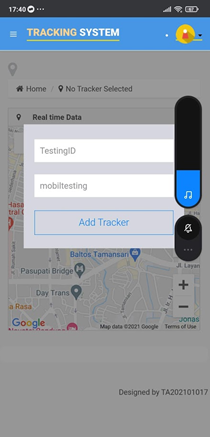
\includegraphics[width=0.2\textwidth]{pairingsuccess1}
    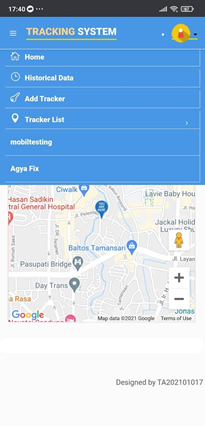
\includegraphics[width=0.2\textwidth]{pairingsuccess2}
    \caption{Pairing Process and Result After Pairing}
    \label{fig1}
\end{figure}

\begin{figure}[htbp]
    \centering
    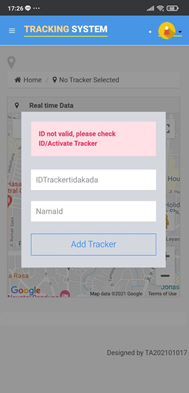
\includegraphics[width=0.2\textwidth]{pairingfail1}
    \caption{First Layer of Verification for Pairing Process}
    \label{fig1}
\end{figure}
The process itself has 2 stages of verification. The first stage of the verification is to check whether the tracker ID given by the user is a valid tracker ID that has been connected to the network. This is done by checking the availability 
of the document with the tracker ID that has been submitted, and if the document cannot be found, a message will be shown stating that the either the Tracker ID is invalid, or the Tracker device has not been turned on for 1 minute. The second level 
of verification involves checking if the Tracker has previously been paired to an account. This is done by checking whether the 'owner' field exists in a document named after the submitted Tracker ID. If the 'owner' field exists, the user interface will return a message 
to re-submit a Tracker ID that has not been paired before. 
\begin{figure}[htbp]
    \centering
    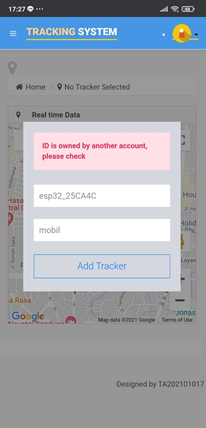
\includegraphics[width=0.2\textwidth]{pairingfail2}
    \caption{Second Layer of Verification for Pairing Process}
    \label{fig1}
\end{figure}

\subsection{Real time Tracking and Historical Location Data Acquisition}
Real time location data acquisition is possible through the Dashboard page. The user will first choose which Tracker Device. The chosen Tracker Device will then be selected, and the latest recorded location will be displayed in Google Maps interface, along with the location of the user 
accessing the application. The user will then be able to choose to turn on real time tracking to get the latest location data from a button element available in the Dashboard. Once it is selected, it will create a change in data in Firestore Database by changing the value of the 'ReqReal' field from '0' to '1', where it will be detected by a Cloud Function that is designed to detect changes in the document. 
This will then send a new configuration to the device, telling the device to turn on real time tracking, where it will provide an update at a rate of every 10 seconds, provided that GPS data is provided by the receiver.

\begin{figure}[htbp]
    \centering
    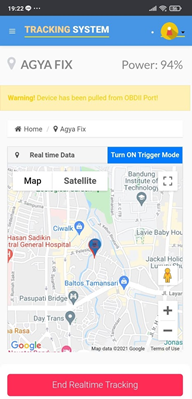
\includegraphics[width=0.2\textwidth]{realtimeon}
    \caption{Real Time Tracking Turned on in Dashboard}
    \label{fig1}
\end{figure}
Aside from real time location data, the tracker device will also send historical location data automatically without prompt, providing the user with extra precaution in the case that they forgot to enable theft detection mode. Historical data can be accessed in the History page of the application. The user will need to choose a paired Tracker device in the menu, 
where they will be able to view all of the available historical data in Google Maps as a collective unit. When the user selects one of the pins available in the map, they will see the time it was recorded in database. The user may also choose one data to be displayed in the map, eliminating all of the collective pins that are needed. This is also shown alongside the location of the user 
to help give a comparison between the user and the location data that is selected.
\begin{figure}[htbp]
    \centering
    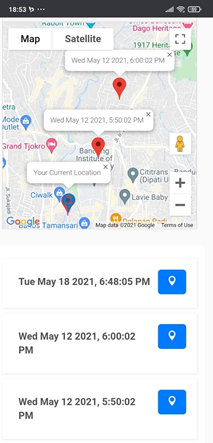
\includegraphics[width=0.2\textwidth]{history1}
    \caption{Initial Historical Data Display After Selecting Tracker}
    \label{fig1}
\end{figure}
\begin{figure}[htbp]
    \centering
    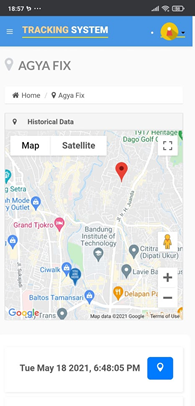
\includegraphics[width=0.2\textwidth]{history2}
    \caption{Historical Data Display After Selecting Individual Data}
    \label{fig1}
\end{figure}

\subsection{Theft Detection Simulation}
Theft detection is possible by turning on theft monitoring configuration, by pressing the 'Turn ON Trigger Mode' button in the dashboard Page. Turning on this future will change the 'Trigger' field from '0' to '1', and this changed will be detected by a Cloud Function, and will instruct the device to change configuration and monitor for scenarios of car theft. These scenarios include:
\begin{itemize}
\item Vehicle engine is turned on
\item Vehicle has changed position to a distance of 50 meters from its original location.
\end{itemize}
\begin{figure}[htbp]
    \centering
    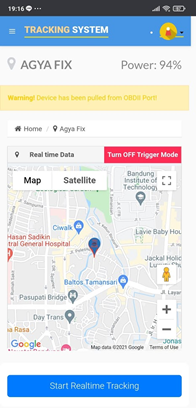
\includegraphics[width=0.2\textwidth]{triggeron}
    \caption{Theft Monitoring Turned on in Dashboard}
    \label{fig1}
\end{figure}
When theft is detected through these two scenarios, it will send a push notification the user's device, while also displaying a message to remind the user of the situation when they access the Dashboard page.
\begin{figure}[htbp]
    \centering
    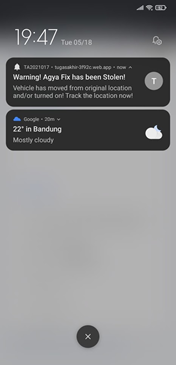
\includegraphics[width=0.2\textwidth]{notif1}
    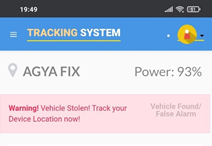
\includegraphics[width=0.25\textwidth]{notif2}
    \caption{Notification and Displayed Message when Theft is Detected}
    \label{fig1}
\end{figure}
Detecting state of engine turning on will use the OBDII port as explained previously. If the OBDII port is unplugged, there will be a different warning given to the user as shown. This notification will be sent even when Trigger Mode is off, and will give an extra layer of precaution, or in the other words acts as a failsafe for all the safety features that are available.
\begin{figure}[htbp]
    \centering
    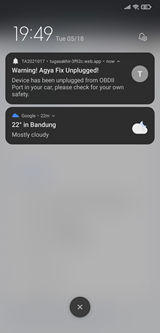
\includegraphics[width=0.2\textwidth]{notif3}
    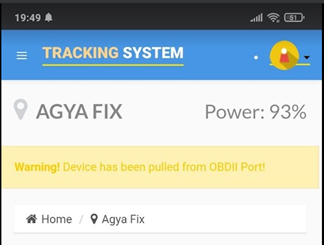
\includegraphics[width=0.25\textwidth]{notif4}
    \caption{Notification and Displayed Message when Device is Unplugged from OBDII Port}
    \label{fig1}
\end{figure}

\section{Conclusion}
A system has been designed that has been able to incorporate GPS and GPRS technology to track location of passenger cars. The system is also able to detect an act of theft through 2 predefined scenarios, which are when engine is turned on and when the vehicle has moved 50 meters from its original position. 
The user is able to access all of the information given by the Tracker through a user interface designed as a Progressive Web App which enables features such as push notifications to be possible in a web-based application. Communication between Tracker and User Interface is fulfilled with Google Cloud Solutions, consisting of Google IoT Core, Cloud Functions, and Firebase Firestore. 
Implementation is possible in passenger cars with OBDII Port, where engine-turn on data and main power is acquired. Backup power is provided by a battery pack for situations where OBDII Port is unplugged, which will also be informed to the user via push notifications. 


\section{Future Development}
This system can be enhanced further by implementing the use of 4G LTE instead of GPRS once the components are available for a more economical price point. Any technology that can be used is to use Narrowband-IoT (NB-IoT) as a means of communications once the infrastructure is available to be used for general public in Indonesia. Implementing NB-IoT will allow for less power consumption and enable the device to be powered solely by external power source, like a battery pack, and enable more reliable 
mobile network connection. Another development would be offering this system to motorcycles, by changing the interfacing format to the vehicle from OBDII to other means.


\bibliographystyle{IEEEtran}
\bibliography{references}

\end{document}
